\documentclass{beamer}
\usepackage[utf8]{inputenc}
\usepackage{tikz} % For semi-transparent background blocks
\usepackage{hyperref}
\usepackage{multimedia}
\usepackage{ulem}
\usepackage{wasysym}

\usepackage{pbox}

%%%%%%%%%%%%%%%%%%%%%%%%%%%%%%%%%%%%%%%%%%%%%%%%%%%%%%%%%%%%%%%%%%%
% Style modifications
%%%%%%%%%%%%%%%%%%%%%%%%%%%%%%%%%%%%%%%%%%%%%%%%%%%%%%%%%%%%%%%%%%%

\usetheme{Berlin}

%%% Fonts %%%

% Change font. Fontspec requires xelatex instead of pdflatex!
% Font catalog: http://www.tug.dk/FontCatalogue/
\usepackage{fontspec}

%\setsansfont{Comfortaa}
%\setsansfont{DejaVu Sans}
%\setsansfont{Fira Sans}

% Use "Fira Sans Light" as the normal font and the "Fira Sans" for
% bold fonts
\setsansfont[
  ItalicFont={Fira Sans Light Italic},
  BoldFont={Fira Sans},
  BoldItalicFont={Fira Sans Italic}]{Fira Sans Light}

\setbeamerfont{title}{size=\huge, series=\bfseries}
\setbeamerfont{frametitle}{size=\large, series=\bfseries}
\setbeamerfont{block body}{size=\huge}

%%% Slide template %%%

\setbeamertemplate{frames}[default]

% Empty headline / footline
\setbeamertemplate{headline}{}
\setbeamertemplate{footline}{}

% Remove navigation icons
\setbeamertemplate{navigation symbols}{}

%%% Colors %%%

\usecolortheme{crane}

\definecolor{lightgray}{RGB}{245,245,245}
\definecolor{darkgray}{RGB}{45,45,45}

% Use the slide background in block environments                                                                                                      

\setbeamercolor{title}{fg=white,bg=darkgray}

\setbeamertemplate{blocks}[default]
\setbeamercolor{block title}{bg=}
\setbeamercolor{block body}{bg=lightgray}
\setbeamercolor{frametitle}{fg=white,bg=darkgray}
\setbeamercolor{itemize item}{fg=darkgray}
\setbeamertemplate{itemize items}[circle]
\setbeamercolor{section number projected}{bg=darkgray,fg=white}
\setbeamercolor{section in toc}{fg=darkgray}
\setbeamercolor{subsection in toc}{fg=darkgray}

\addtobeamertemplate{block begin}{\pgfsetfillopacity{0.8}}{\pgfsetfillopacity{1}}
\addtobeamertemplate{frametitle}{\pgfsetfillopacity{0.8}}{\pgfsetfillopacity{1}}
\addtobeamertemplate{title page}{\pgfsetfillopacity{0.8}}{\pgfsetfillopacity{1}}

%%% Misc %%%

% Command to place the test (e.g. citation) in the center of the footer
\newcommand{\setfootercentertext}[1]{
\setbeamertemplate{footline}{
  \hspace*{\fill}
  \raisebox{3mm}[0mm][0mm]{
    \tiny{#1}}\hspace*{\fill}}
}

%%%%%%%%%%%%%%%%%%%%%%%%%%%%%%%%%%%%%%%%%%%%%%%%%%%%%%%%%%%%%%%%%%%
% Content
%%%%%%%%%%%%%%%%%%%%%%%%%%%%%%%%%%%%%%%%%%%%%%%%%%%%%%%%%%%%%%%%%%%

%------------------------------------------------------------------------------
\title{What is good scientific practice\\for research software?}
%------------------------------------------------------------------------------

%\subtitle{Working Group Research Software}

\author{\small Konrad U. Förstner\\
  \vspace{0.5cm}
  \textcolor{orange}{@konradfoerstner}}

\institute{University of Würzburg}

\date{\scriptsize May 10$^{th}$, 2017}

\logo{
  \href{https://creativecommons.org/licenses/by/4.0/}{
    
\includegraphics[width=0.88cm]{images/creative_commons_attribute.png}}}
\begin{document}
\begin{frame}{}
  \titlepage
\end{frame}
\logo{}

\setbeamertemplate{background}{}

% Symbiosis of technology and science
% Tools - Science
% examples: Telescope / Microscope
\begin{frame}
  \frametitle{}
  \begin{block}{}
    \begin{center}
      Science $\rightleftarrows$ Technology
      \end{center}
  \end{block}
\end{frame}

% Telescope
\setbeamertemplate{background}{
  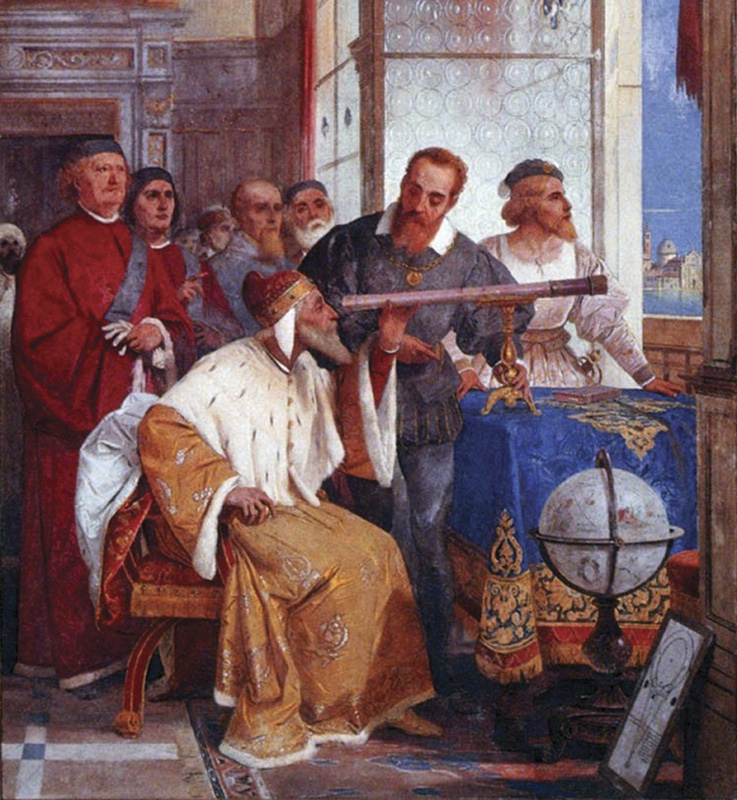
\includegraphics[width=\paperwidth]{images/Bertini_fresco_of_Galileo_Galilei_and_Doge_of_Venice.jpg}}
\setbeamertemplate{footline}{\raisebox{2mm}[2mm][2mm]{\Tiny{
      \href{https://commons.wikimedia.org/wiki/File:Bertini_fresco_of_Galileo_Galilei_and_Doge_of_Venice.jpg}{
        https://commons.wikimedia.org/wiki/File:Bertini\_fresco\_of\_Galileo\_Galilei\_and\_Doge\_of\_Venice.jpg} - PD}}}
\begin{frame}
\end{frame}

% Microscope
\setbeamertemplate{background}{
  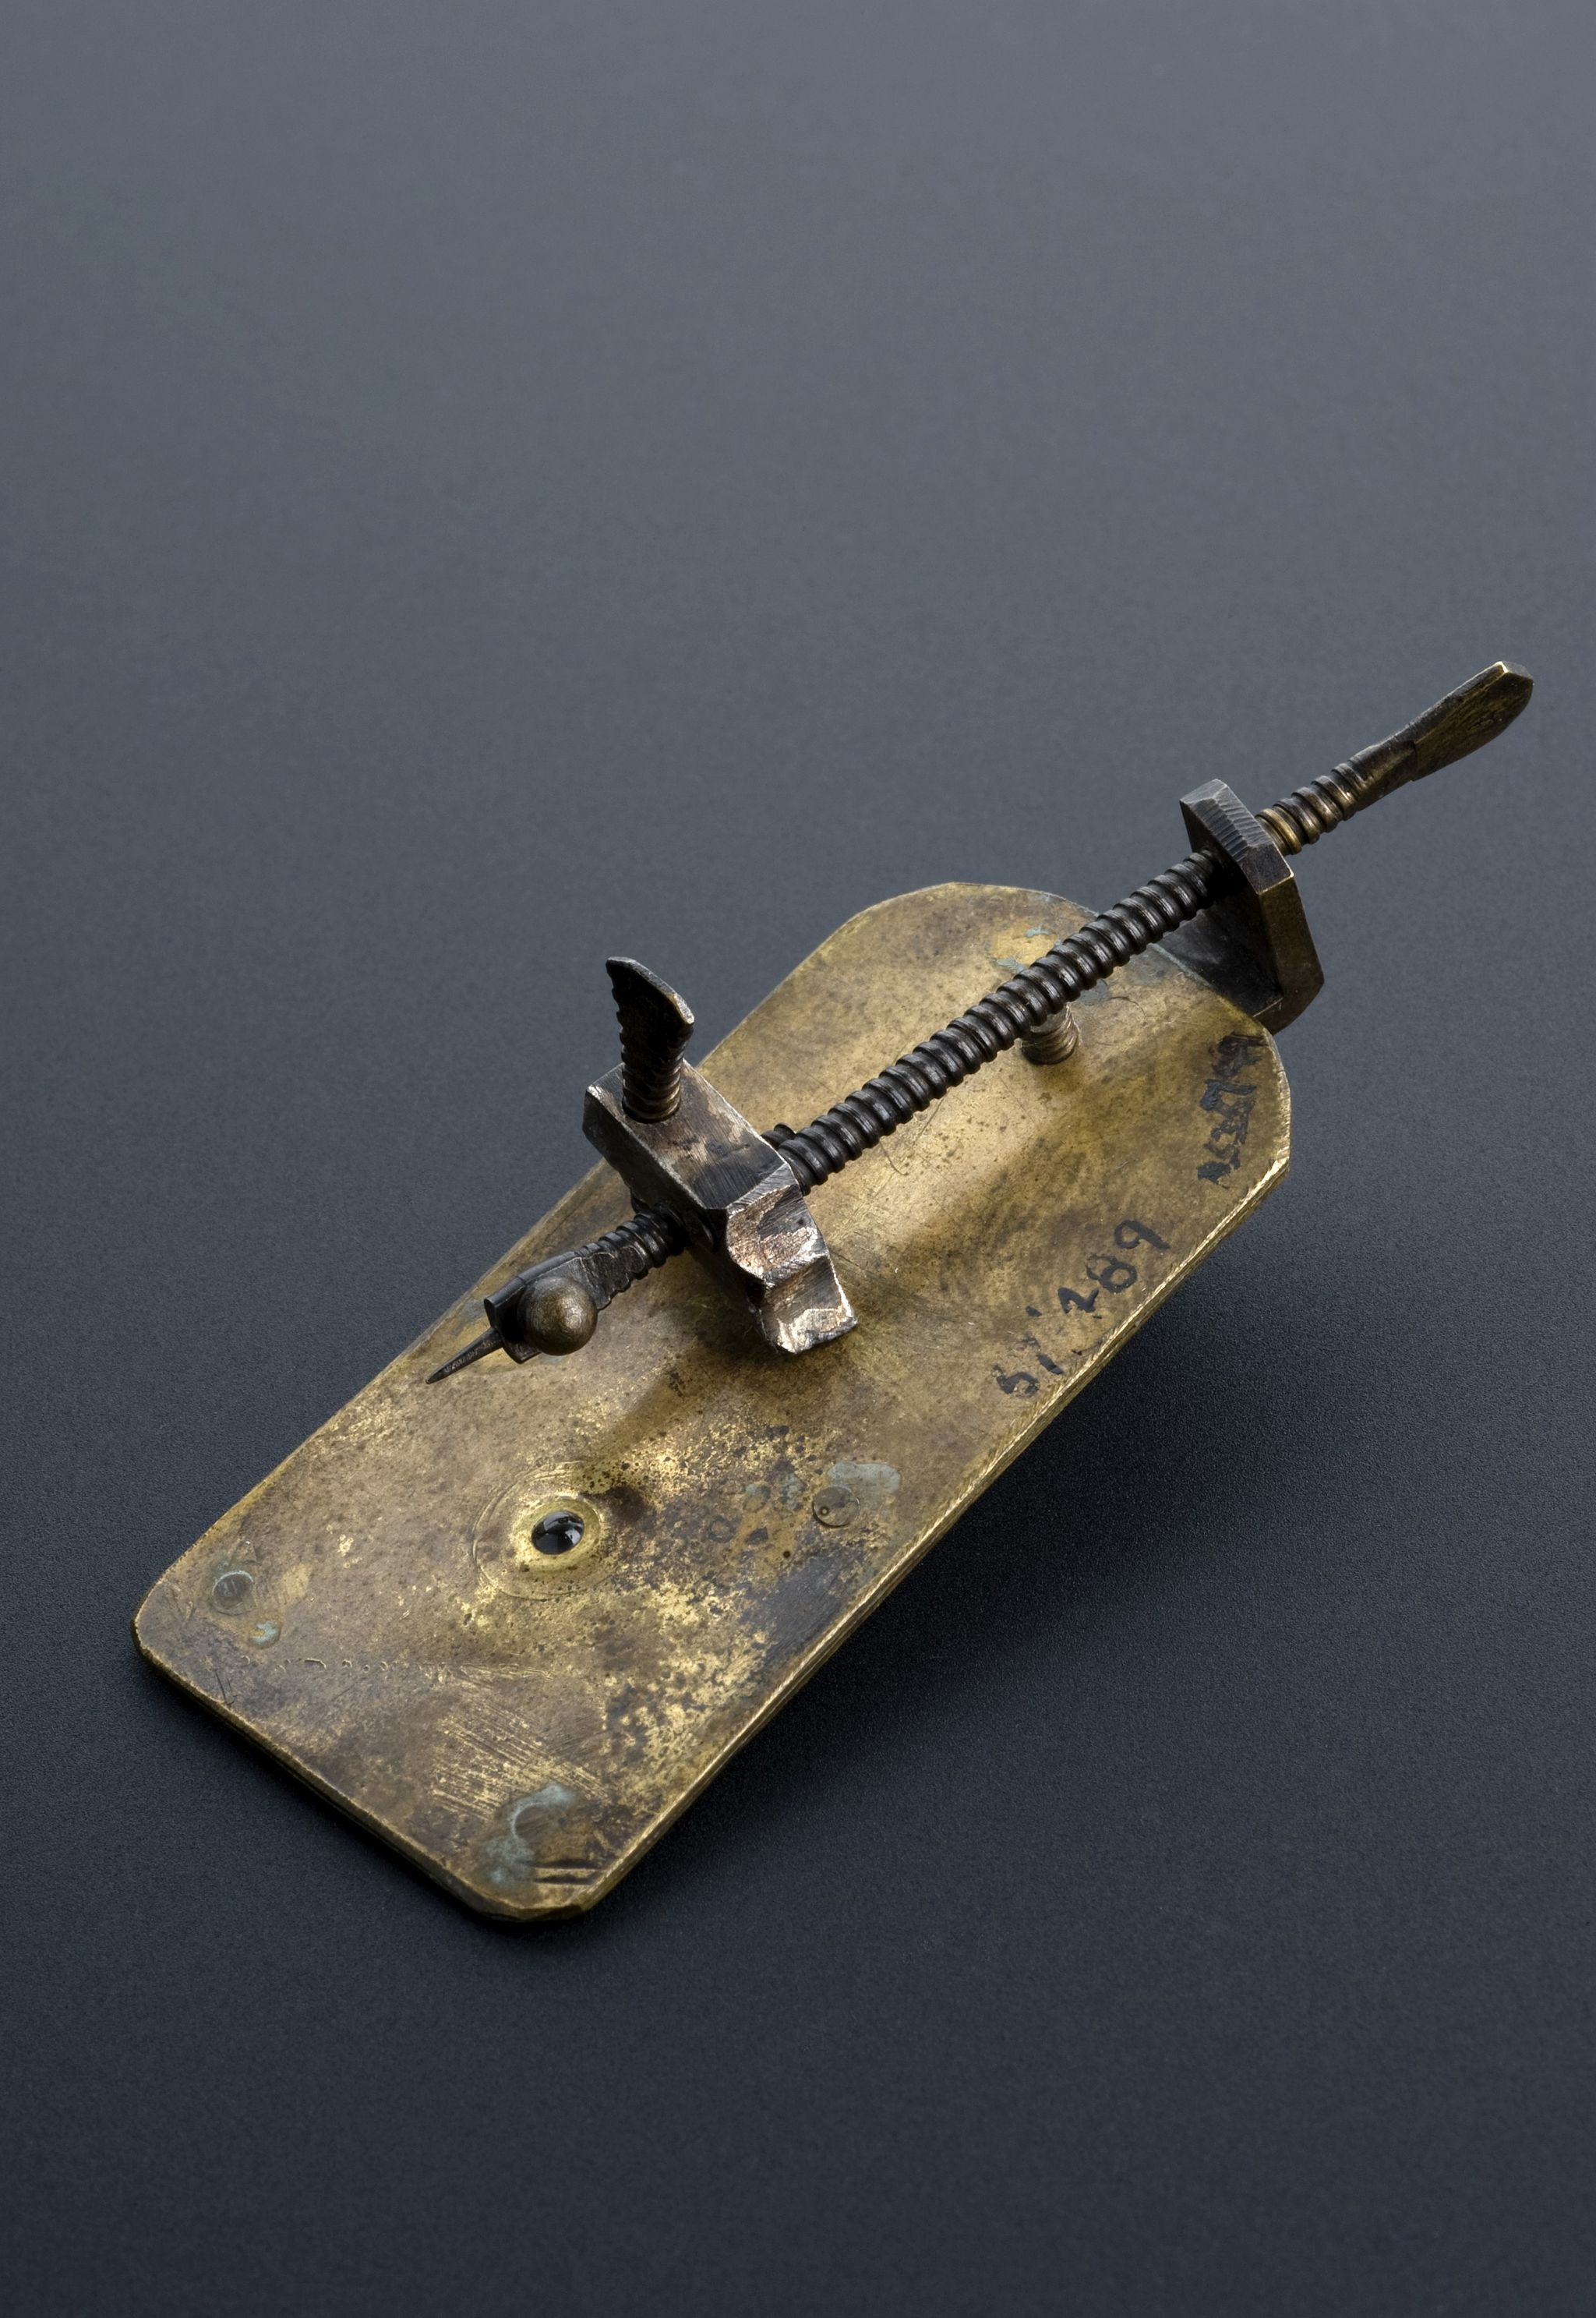
\includegraphics[width=\paperwidth,trim=0 0 0 210,clip]{images/2048px-Leeuwenhoek_simple_microscope_(copy),_Leyden,_1901-1930_Wellcome_L0057739.jpg}}
\setbeamertemplate{footline}{\raisebox{2mm}[2mm][2mm]{\Tiny{
      \href{https://commons.wikimedia.org/wiki/File:Leeuwenhoek_simple_microscope_(copy),_Leyden,_1901-1930_Wellcome_L0057739.jpg}{
        https://commons.wikimedia.org/wiki/File:Leeuwenhoek\_simple\_microscope\_(copy),\_Leyden,\_1901-1930\_Wellcome\_L0057739.jpg}
      - CC-By by Wiki Commons User \href{https://commons.wikimedia.org/wiki/User:Fæ}{Fæ}}}}
\begin{frame}
\end{frame}

% Sofware - ubiquitary 
\setbeamertemplate{background}{
  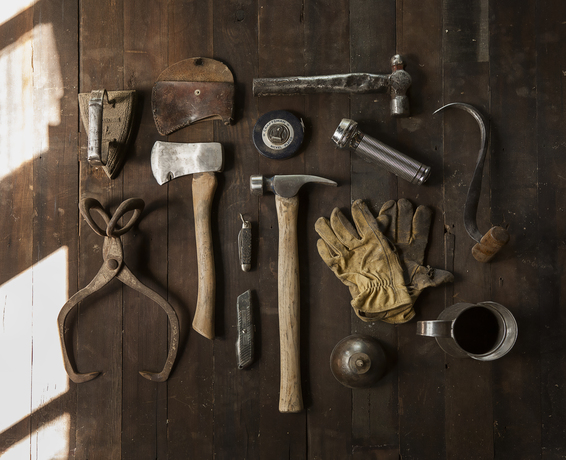
\includegraphics[width=\paperwidth]{images/Tools_by_Todd_Quackenbush.jpg}}
\setbeamertemplate{footline}{\raisebox{2mm}[2mm][2mm]{\Tiny{
      \href{https://unsplash.com/@toddquackenbush?photo=IClZBVw5W5A}{
        https://unsplash.com/@toddquackenbush?photo=IClZBVw5W5A} - PD}}}
\begin{frame}
  \pause  
  \begin{block}{}
    \begin{center}
      Software\\- an ubiquitary research tool
    \end{center}
  \end{block}  
\end{frame}

% Desktop application
\setbeamertemplate{background}{
  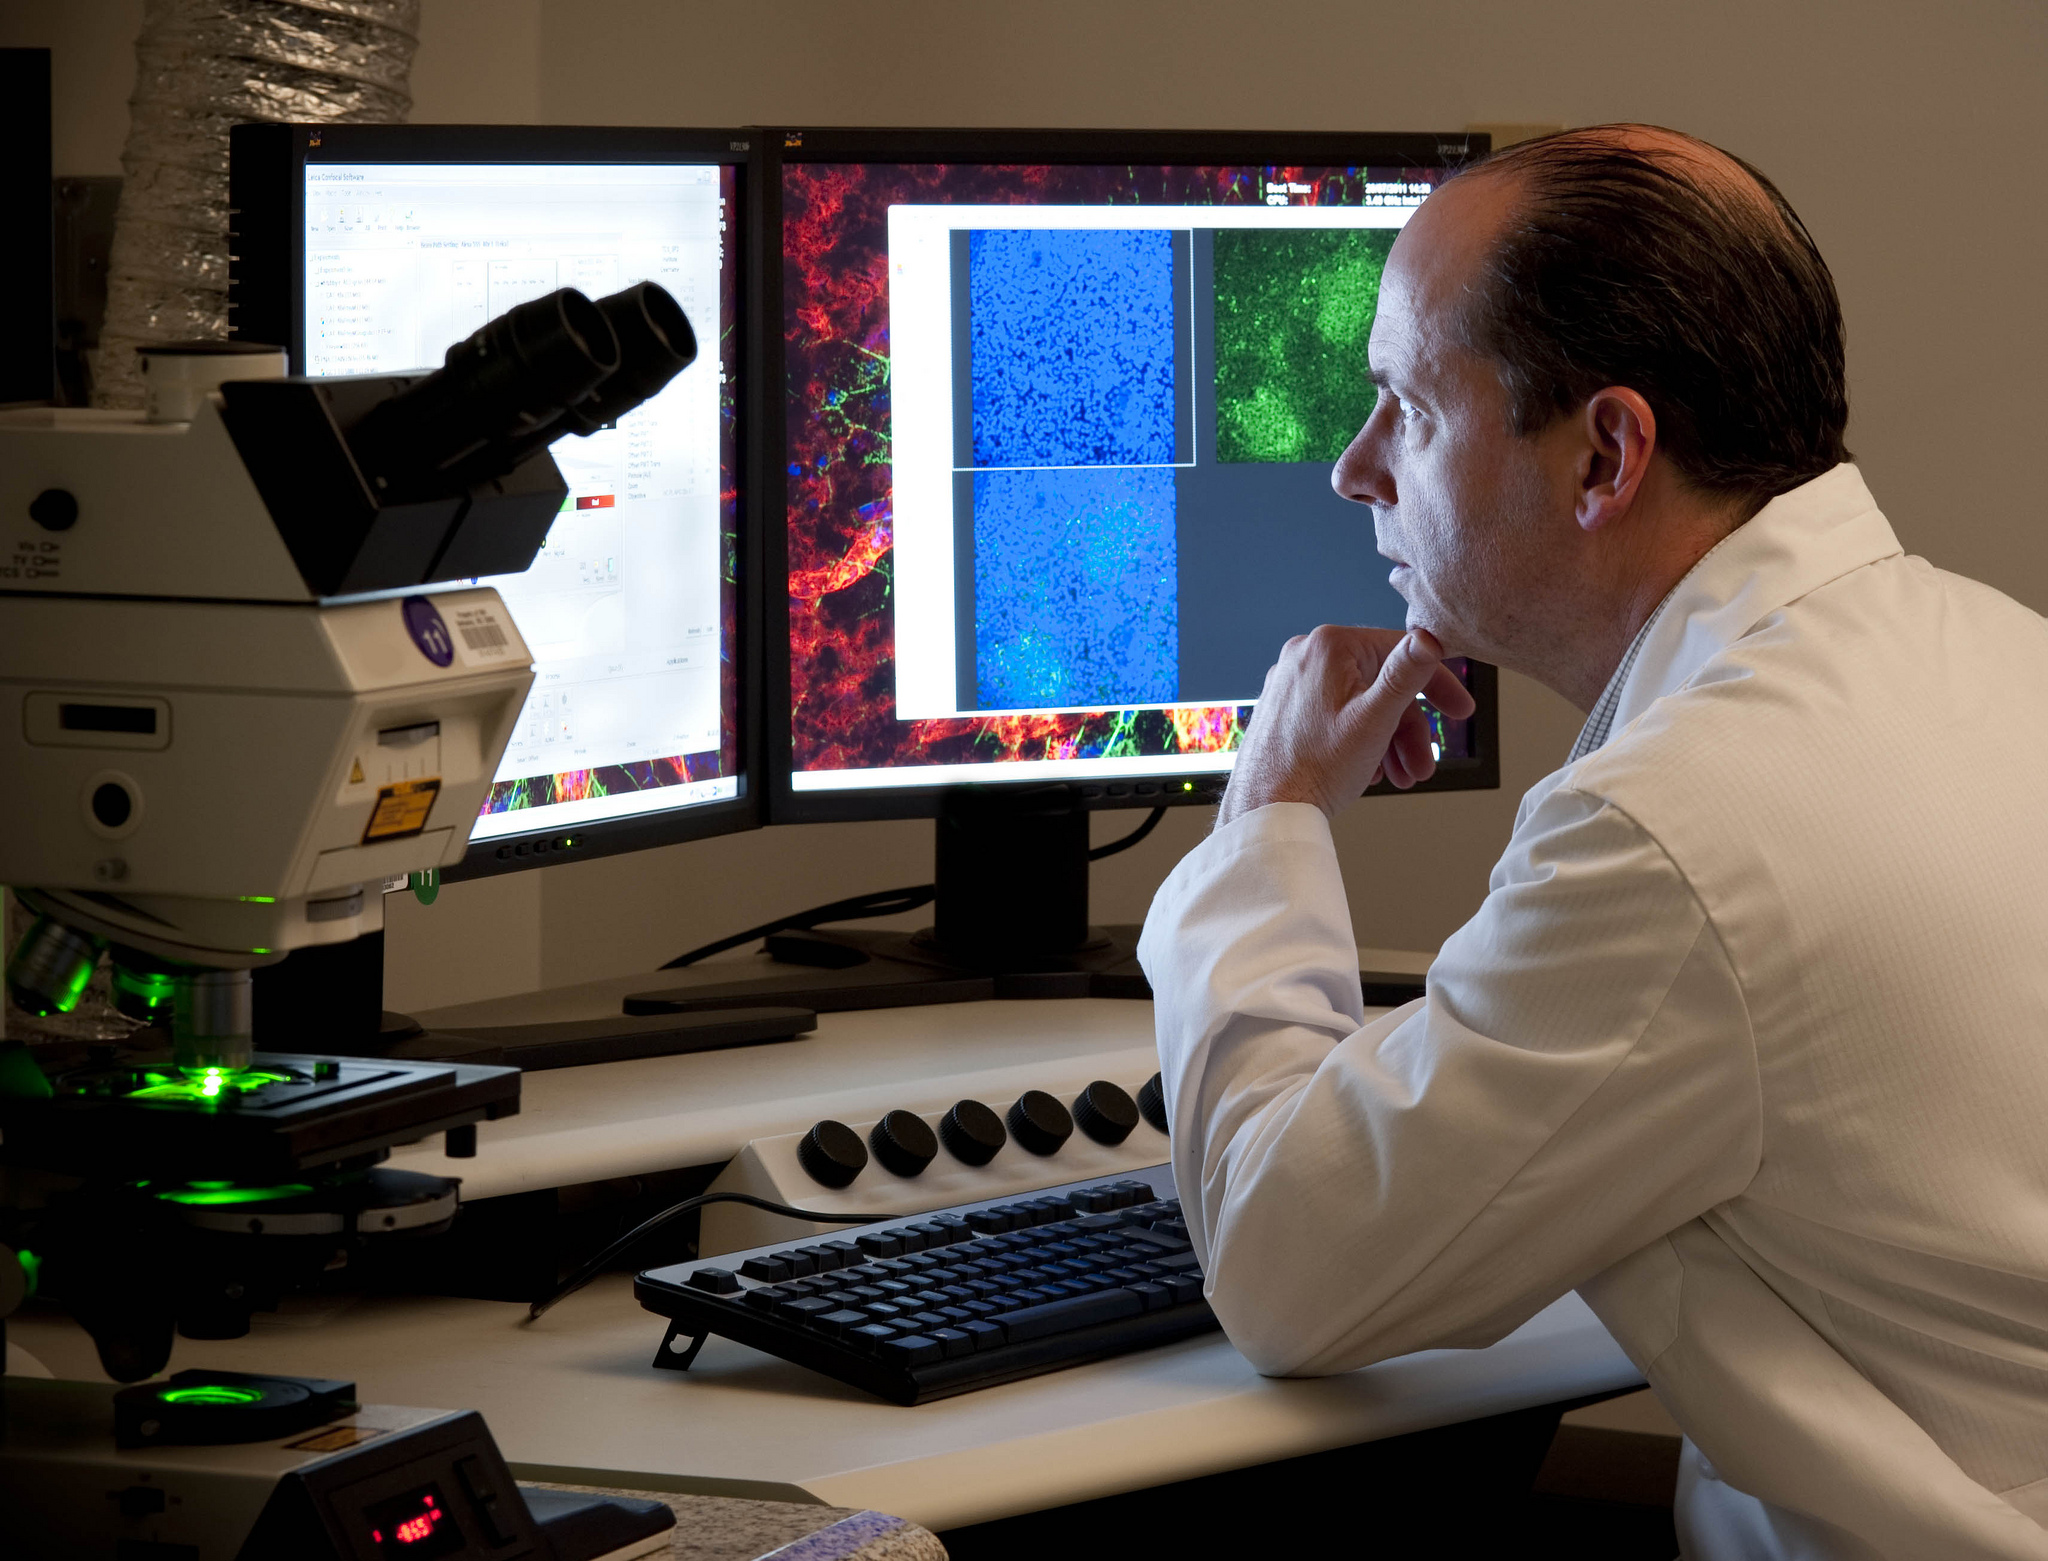
\includegraphics[width=\paperwidth]{images/Flickr_National_Eye_Institute_9955408263.jpg}}
\setbeamertemplate{footline}{\raisebox{2mm}[2mm][2mm]{\Tiny{https://www.flickr.com/photos/80030261@N06/9955408263}{
      https://www.flickr.com/photos/80030261@N06/9955408263}
    - CC-BY \href{https://www.flickr.com/photos/nationaleyeinstitute}{nationaleyeinstitute}}}
\begin{frame}
\end{frame}

% HPC calculation
\setbeamertemplate{background}{
  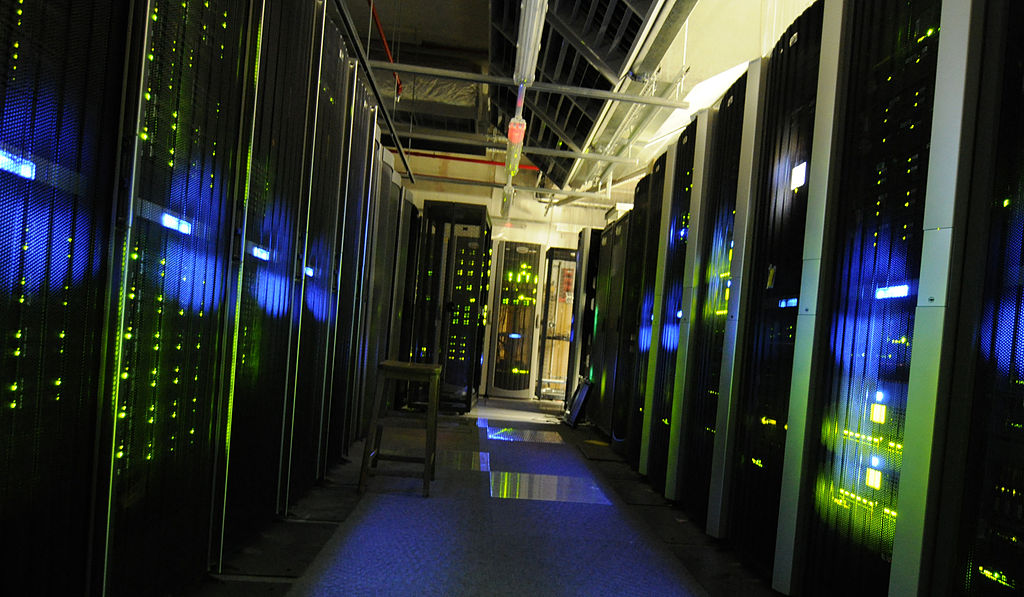
\includegraphics[height=\paperheight]{images/1024px-A_view_of_the_server_room_at_The_National_Archives.jpg}}
\setbeamertemplate{footline}{\raisebox{2mm}[2mm][2mm]{\Tiny{https://www.flickr.com/photos/80030261@N06/9955408263}{
      https://www.flickr.com/photos/80030261@N06/9955408263}
    - CC-By by Wiki Commons User \href{https://commons.wikimedia.org/w/index.php?title=User:EduVolunteer}{EduVolunteer}}}
\begin{frame}
\end{frame}


\setbeamertemplate{background}{}
\setbeamertemplate{footline}{}

\begin{frame}
  \frametitle{}
  \begin{block}{}
    \begin{center}
      Research needs Software
      \end{center}
  \end{block}
\end{frame}

\setbeamertemplate{background}{}
\setbeamertemplate{footline}{}
\begin{frame}
  \frametitle{}
  \begin{block}{}
    \begin{center}
      Should be part of / equivalent to Material and Methodes of a publication
      \end{center}
  \end{block}
\end{frame}

\setbeamertemplate{background}{}
\setbeamertemplate{footline}{}
\begin{frame}
  \frametitle{}
  \begin{center}
    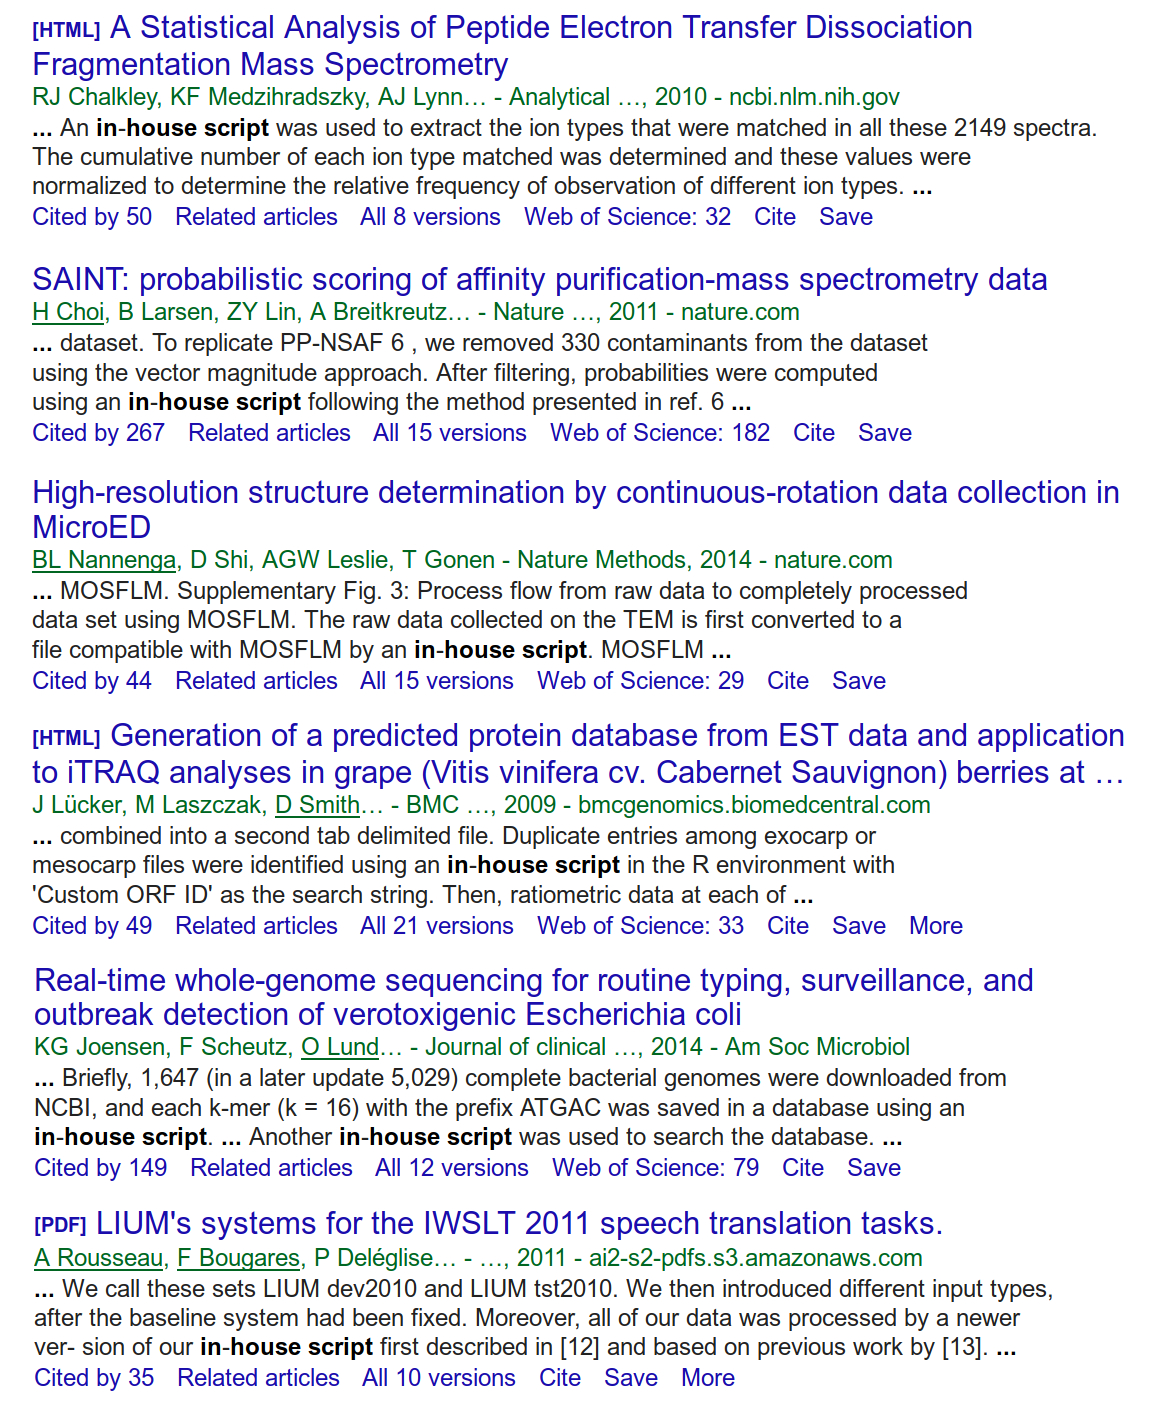
\includegraphics[height=8cm]{images/In-house_script.jpg}
  \end{center}
\end{frame}

\setbeamertemplate{background}{}
\setbeamertemplate{footline}{}
\begin{frame}
  \frametitle{}
  \begin{block}{}
    \begin{center}
      Still it is widely neglected by the majority of researchers,
      journals, funders, politicians.
      \end{center}
  \end{block}
\end{frame}

% But this is changing, this confernce is a proof of this
% Several iniatives have been lauchend
\setbeamertemplate{background}{
  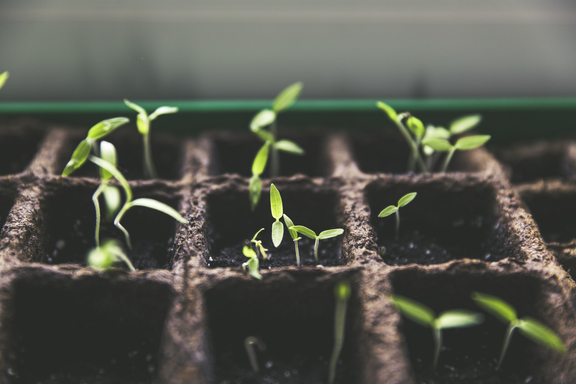
\includegraphics[height=\paperheight]{images/Sprout_by_Markus-Spiske.jpg}}
\setbeamertemplate{footline}{\raisebox{2mm}[2mm][2mm]{\Tiny{
      \href{https://unsplash.com/photos/vrbZVyX2k4I}{
        https://unsplash.com/photos/vrbZVyX2k4I} - PD}}}
\begin{frame}
  \begin{block}{}
    \begin{center}
      Several iniatives has been launched
    \end{center}
  \end{block}
\end{frame}

\begin{frame}
  \frametitle{}
  \begin{block}{}
    \begin{itemize}
    \item SSI (already 2008!)
    \item Free Software Foundation Europe published a position paper
      for the endorsement of Free Software and Open Standards in
      Horizon 2020 and all publicly-funded research
    \item 
    \item DFG program "Research Software Sustainability" (7M €, 130)
    \item de-RSE (de-rse.org) founded
    \item Helmholtz Association Task Group "Access to and re-use of
      research software" launchen and organized a workshop about
      research software.
    \end{itemize}    
  \end{block}
\end{frame}

\setbeamertemplate{background}{}
\setbeamertemplate{footline}{}
\begin{frame}
  \frametitle{}
  \begin{center}

    Priority Initiative "Digital Information"\\
    of the\\
    Alliance of Science Organisations in Germany\\
    \ \\
    % TMP
    \includegraphics[height=2cm]{logo_allianz.png}\\
    \ \\
    Foudend in 2008
    
  \end{center}
\end{frame}


\setbeamertemplate{background}{}
\setbeamertemplate{footline}{}
\begin{frame}
  \frametitle{}
    \begin{block}{}
      \begin{center}
        Priority areas
        \begin{itemize}
        \item Open Access (DEAL!)
        \item Research Data
        \item Virtual Research Environments
        \item National Licensing
        \item National Hosting Strategy
        \item Legal Frameworks
        \end{itemize}
      \end{center}
    \end{block}
\end{frame}


\setbeamertemplate{background}{}
\setbeamertemplate{footline}{}
\begin{frame}
  \frametitle{}
    \begin{block}{}
      \begin{center}
        Since 2016 - Ad-hoc working group "Research Software"
      \end{center}
    \end{block}
\end{frame}


\setbeamertemplate{background}{}
\setbeamertemplate{footline}{}
\begin{frame}
  \frametitle{}
  \begin{tabular}{lr}
    Mathias Bornschein & Ressortforschung des Bundes\\
    Dr. Matthias Katerbow & DFG \\
    Dr. Michael Erben-Russ & Fraunhofer-Gesellschaft \\
    Dr. Bernadette Fritzsch & Helmholtz-Gemeinschaft \\
    Dr. Uwe Konrad & Helmholtz-Gemeinschaft\\
    Dr. Georg Feulner & Leibniz-Gemeinschaft\\
    Dr. Jürgen Fuhrmann & Leibniz-Gemeinschaft\\
    Michael Franke & Max-Planck-Gesellschaft\\
    Stephan Janosch & Max-Planck-Gesellschaft\\
    Prof. Dr. Andreas Zeller & DFG\\
    Prof. Dr. Björn Brembs & HRK\\
    Dr. Konrad Förstner & HRK\\
  \end{tabular}
\end{frame}

\setbeamertemplate{background}{}
\setbeamertemplate{footline}{}
\begin{frame}
  \frametitle{}
  \begin{block}{}
    Guiding idea\\
    \ \\The concept of Good Scientific Practice (GSP) must be also applied to
    research software.
  \end{block}
\end{frame}

\setbeamertemplate{background}{}
\setbeamertemplate{footline}{}
\begin{frame}
  \frametitle{}
  \begin{block}{}
    Confirmability, reproducibility, transparency and quality muss be
    part of of the development and usage of research software.\\
    \ \\
    Re-use must be faciliated.
  \end{block}
\end{frame}

\begin{frame}
  \frametitle{}
  \begin{block}{}
    \begin{center}
      Software as three "digital tools" of scientific research
      \begin{itemize}
      \item Small tools individually written by the researches, Source Code!
      \item Software applications
      \item Services
      \end{itemize}
    \end{center}
  \end{block}
\end{frame}



\begin{frame}
  \frametitle{}
  \begin{block}{}
    Software as research output
    \begin{center}
      \begin{itemize}
      \item Quality assurance and standards
      \item Publication and Archiving
      \item Citation
      \item Reuse
      \end{itemize}
    \end{center}
  \end{block}
\end{frame}

\begin{frame}
  \frametitle{}
  \begin{block}{}
    Sustainable development of software
    \begin{center}
      \begin{itemize}
      \item From a research project to a application
      \item Licenses
      \item Funding
      \end{itemize}
    \end{center}
  \end{block}
\end{frame}


\begin{frame}
  \frametitle{}
  \begin{block}{}
    Sustainavle development of software
    \begin{center}
      \begin{itemize}
      \item From a research project to a application
      \item Licenses
      \item Funding
      \end{itemize}
    \end{center}
  \end{block}
\end{frame}





\begin{frame}
  \frametitle{}
  \begin{block}{}
    Open for input and offer to collaborate
  \end{block}
\end{frame}


\begin{frame}
  \frametitle{}
  \begin{block}{}
    \begin{center}
      Thank you
      \end{center}    
  \end{block}
\end{frame}



\end{document}
